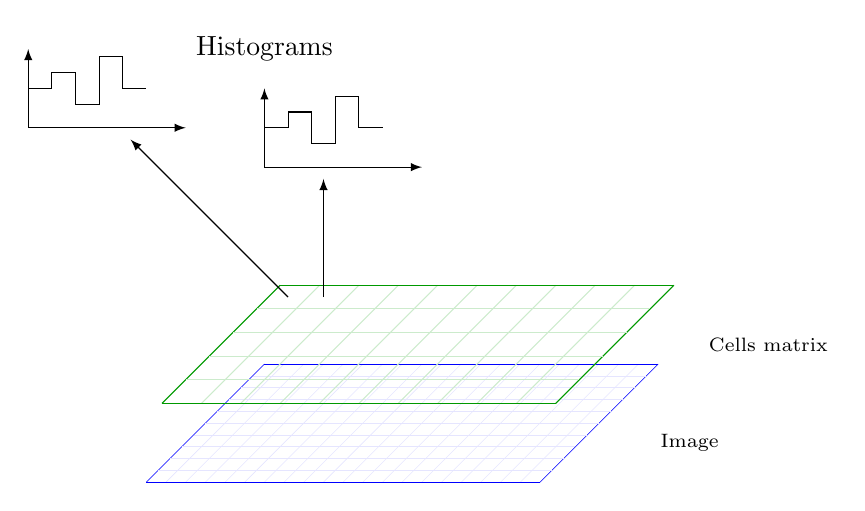
\begin{tikzpicture}[scale=1]

\foreach \x in {0,0.25,0.5,...,5} \draw[color=blue!10,very thin] (\x,0)--+(-1.5,-1.5);
\foreach \x in {0,5} \draw[color=blue,very thin] (\x,0)--+(-1.5,-1.5);

\foreach \y in {0,0.15,0.3,...,1.6 } \draw[color=blue!10,very thin] (-1*\y,-\y)--+(5,0);
\foreach \y in {0,1.5 } \draw[color=blue,very thin] (-1*\y,-\y)--+(5,0);

\node[] at (5.4,-1){{\scriptsize Image}};

\foreach \x in {0,0.5,1,...,5} \draw[color=green!60!black!20,thin] (\x+0.2,0+1)--+(-1.5,-1.5);
\foreach \x in {0,5} \draw[color=green!60!black,thin] (\x+0.2,0+1)--+(-1.5,-1.5);

\foreach \y in {0,0.3,0.6,...,1.6 } \draw[color=green!60!black!20,thin] (-1*\y+0.2,-\y+1)--+(5,0);
\foreach \y in {0,1.5 } \draw[color=green!60!black,thin] (-1*\y+0.2,-\y+1)--+(5,0);
\node[] at (6.4,0.25){{\scriptsize Cells matrix}};


\draw[-latex](0.3,0.85)--+(-2,2);
\draw[-latex](-3,3)--+(2,0);
\draw[-latex](-3,3)--+(0,1);
\draw[](-3,3.5)--+(0.3,0)--+(0.3,0.2)--+(0.6,0.2)--+(0.6,-.2)--+(0.9,-.2)--+(0.9,.4)--+(1.2,.4)--+(1.2,0)--+(1.5,0);

%
%
\draw[-latex](0.75,0.85)--+(0,1.5);
\draw[-latex](0.,2.5)--+(2,0);
  \draw[-latex](0.,2.5)--+(0,1);
  \draw[](0,3)--+(0.3,0)--+(0.3,0.2)--+(0.6,0.2)--+(0.6,-.2)--+(0.9,-.2)--+(0.9,.4)--+(1.2,.4)--+(1.2,0)--+(1.5,0);
  \node[] at (0,4){Histograms};
\end{tikzpicture}
